%% LyX 2.4.3 created this file.  For more info, see https://www.lyx.org/.
%% Do not edit unless you really know what you are doing.
\documentclass[12pt,onecolumn,fleqn,english,compsoc]{IEEEtran}
\usepackage{lmodern}
\renewcommand{\sfdefault}{lmss}
\renewcommand{\ttdefault}{lmtt}
\usepackage[T1]{fontenc}
\usepackage{textcomp}
\usepackage[latin9]{inputenc}
\usepackage{parskip}
\usepackage{color}
\usepackage{babel}
\usepackage{amsmath}
\usepackage{amssymb}
\usepackage{graphicx}
\usepackage[bookmarks=true,bookmarksnumbered=true,bookmarksopen=true,bookmarksopenlevel=2,
 breaklinks=false,pdfborder={0 0 0},pdfborderstyle={},backref=false,colorlinks=true]
 {hyperref}
\hypersetup{pdftitle={A simple iterative grid- and density-based Clustering Algorithm},
 pdfauthor={Uwe St�hr},
 pdfsubject={data clustering},
 pdfkeywords={clustering},
 pdfpagelayout=OneColumn,pdfstartview=XYZ,linkcolor=black, citecolor=black}

\makeatletter

%%%%%%%%%%%%%%%%%%%%%%%%%%%%%% LyX specific LaTeX commands.
\newcommand{\noun}[1]{\textsc{#1}}

%%%%%%%%%%%%%%%%%%%%%%%%%%%%%% User specified LaTeX commands.
% enable hyperlinks to subcaptions
\usepackage[figure]{hypcap}
% set caption labels bold and use indentation
\usepackage[labelfont=bf,format=hang]{caption}

% redefine the automatic names for references to labels
\AtBeginDocument{\renewcommand{\ref}[1]{\mbox{\autoref{#1}}}}
\newlength{\abc}
\settowidth{\abc}{\space}
\AtBeginDocument{%
 \renewcommand{\equationautorefname}{\hspace{-\abc}}
 \renewcommand{\itemautorefname}{\hspace{-\abc}}
 \renewcommand{\sectionautorefname}{Sec.\negthinspace}
 \renewcommand{\subsectionautorefname}{Sec.\negthinspace}
 \renewcommand{\subsubsectionautorefname}{Sec.\negthinspace}
 \renewcommand{\figureautorefname}{Fig.\negthinspace}
}

% raises threshold above which floats appear on
% one page alone
\renewcommand{\floatpagefraction}{0.7}

% raises threshold above which floats appear at
% bottom of page
\renewcommand{\bottomfraction}{0.5}

% needed for biblatex
\usepackage{csquotes}

% protect some workds from being hyphenated
\hyphenation{DBSCAN}
\hyphenation{DENCLUE}
\hyphenation{CLIQUE}

\ifdefined\showcaptionsetup
 % Caption package is used. Advise subfig not to load it again.
 \PassOptionsToPackage{caption=false}{subfig}
\fi
\usepackage{subfig}
\makeatother

\usepackage[style=numeric,sorting=none]{biblatex}
\addbibresource{biblio/Clustering.bib}
\begin{document}
\title{A simple iterative grid- and density-based Clustering Algorithm}
\author{\IEEEauthorblockN{Uwe St�hr}

\IEEEauthorblockA{Soloof EOOD, Sofia, Bulgaria\\
Email: research\negthinspace{ }@\negthinspace{ }soloof.com\\
Project Page: \href{https://codeberg.org/Soloof/Iteridense}{https://codeberg.org/Soloof/Iteridense}}\vspace{-3\baselineskip}
}
\maketitle
\begin{abstract}
We introduce \noun{Iteridense}, an iterative clustering algorithm
combining grid-based and density-based methods. It provides two possibilities
to perform the clustering and for both it provides a clear path on
how to change the algorithm's input parameters to achieve suitable
results. We show that \noun{Iteridense} is applicable for datasets
with any dimensionality. \noun{Iteridense} provides shorter computation
times than pure density-based algorithms and that it performs clustering
at least as good to the DBSCAN algorithm. This work enables users
to cluster data in a quick, reliable and objective way based on the
the probability-density of the data.
\end{abstract}


\section{Introduction}

Density-based clustering algorithms have been proven useful for many
practical application. There exists a wide variety of algorithms,
some optimized for particular use cases~\cite{Kriegel2011}. However,
these algorithms have a major drawback -- one needs to evaluate neighboring
points for every data point in the dataset to determine if it is part
of a cluster. This is the case for most density-based clustering algorithms
like PreDeCon~\cite{Boehm2004} or HDBSCAN~\cite{Campello2013}.
Other algorithms that combine grid-based with density-based methods
like DENCLUE~\cite{Hinneburg1998} or CLIQUE\,\cite{Agrawal1998}
don't have this drawback but make assumptions about the shape of the
probability distribution.

Another issue of many clustering algorithms is that as user there
is no clear path on how to change the algorithm's input parameters
to achieve a suitable clustering result. Taking for example the algorithm
DBSCAN~\cite{Ester1996}, it requires to specify the parameter $\epsilon$,
the maximum distance to another core point of a cluster. For many
use cases there is no clear path on how to change $\epsilon$ to get
a suitable result as we will also discuss in this paper.

The algorithm presented in this paper uses both, density-based and
grid-based methods. Its base idea is to work with different probability-density
functions of the dataset and analyzing them in a grid. Therefore even
for small datasets in 2~dimensions the computation can be 10~times
faster than a pure density-based algorithm like DBSCAN. Our algorithm
follows an iterative approach to calculate the probability-density
function and makes no assumptions about the shape of that function.
Therefore it provides a clear path on how to set a start value of
the algorithm's main parameter and how to change it to achieve a certain
result.

\pagebreak{}

\section{Derivation of the Algorithm\label{sec:Derivation-of-the}}

The basic idea of the algorithm is how mountain peak areas are separated
from each other in a geographical relief. Take for example the relief
shown at the left in \ref{fig:Relief-of-a}. To identify areas around
a peak one cuts the relief at a desired height. The cut-off areas
are then the mountain peak areas. For example in \ref{fig:Relief-of-a}\,(a)
the relief was cut at about 2/3 of the maximal height leading to more
than a dozen peak areas. In \ref{fig:Relief-of-a}\,(b) the relief
was cut at about half the maximal size leading to larger areas. By
decreasing the cutting height, the number of areas will become fewer
unless at a zero height the whole relief area is part of a single
mountain area.

\begin{figure}
\begin{centering}
\subfloat[Cut at 2/3 of its maximal height.]{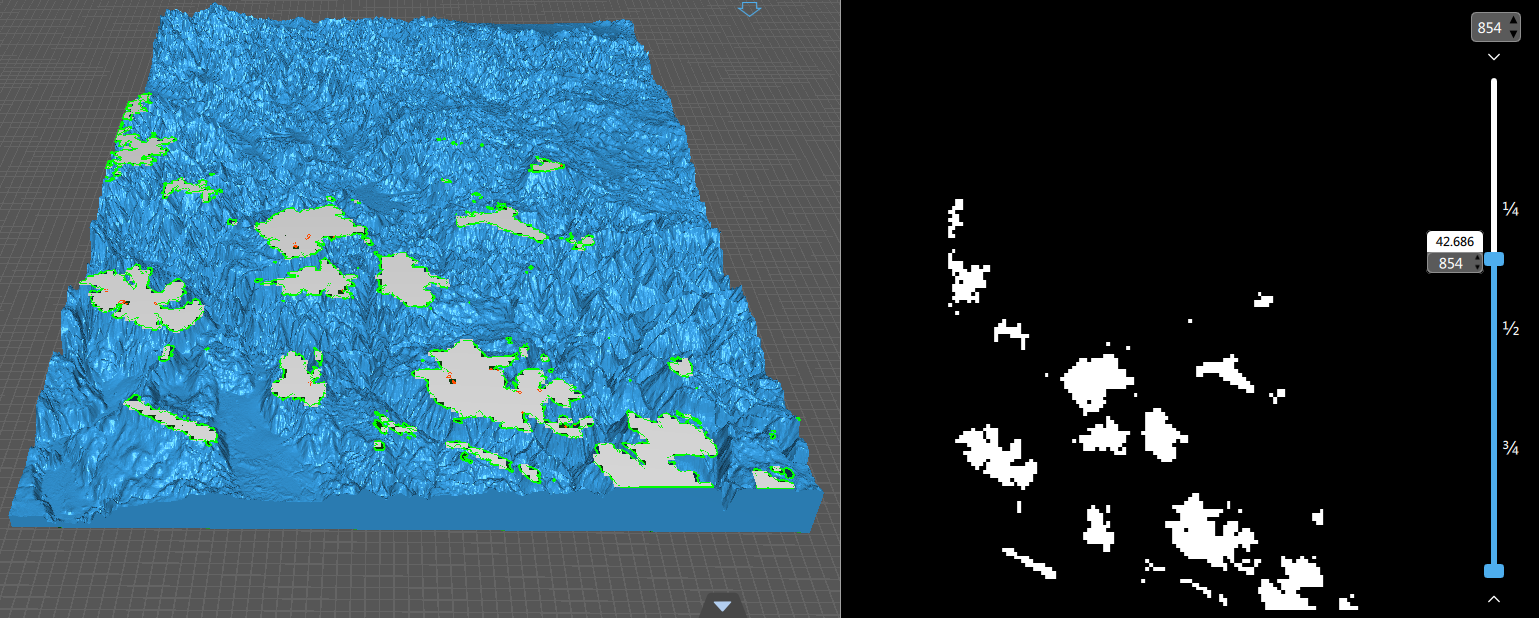
\includegraphics[width=0.75\columnwidth]{clipart/Height-map-layer-854}

}
\par\end{centering}
\begin{centering}
\subfloat[Cut at half of its maximal height.]{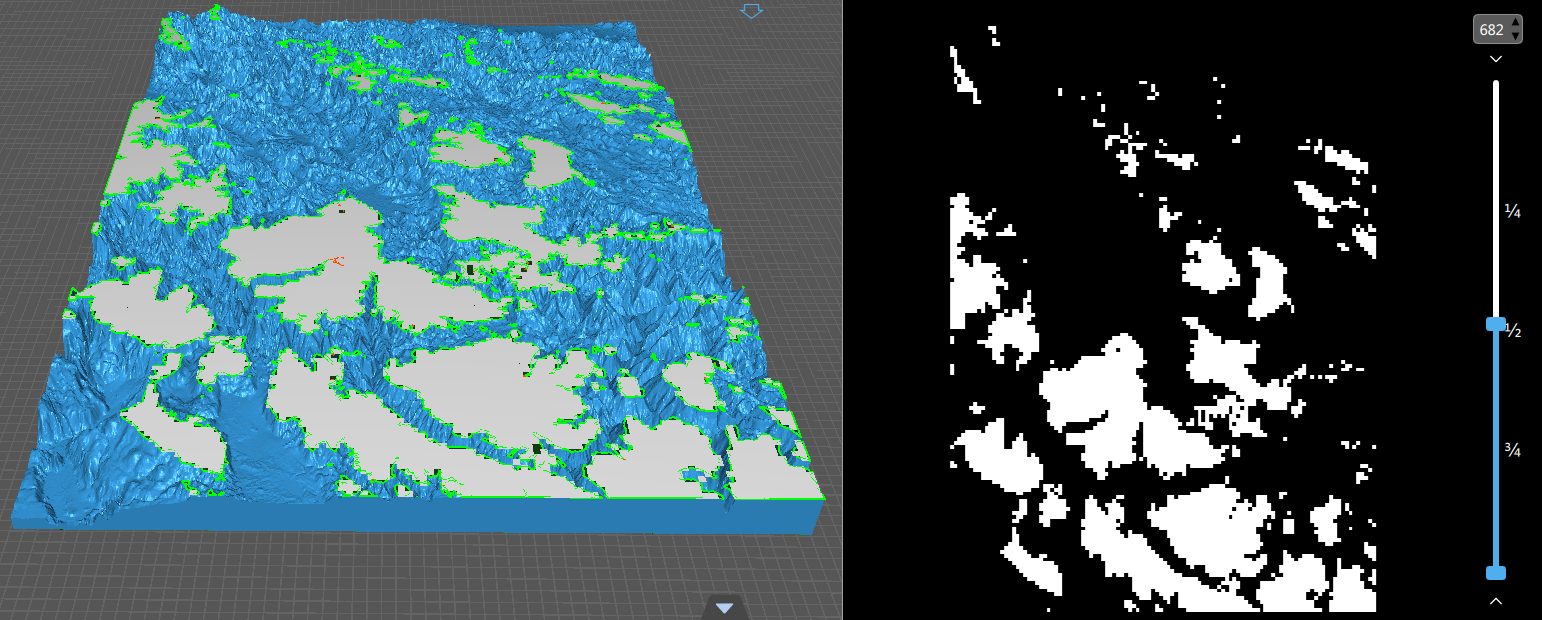
\includegraphics[width=0.75\columnwidth]{clipart/Height-map-layer-682}

}
\par\end{centering}
\caption{\label{fig:Relief-of-a}Relief of a random geographic area cut at
different heights.}
\end{figure}

Translating the height to the density of data points $\rho$ the cut
is made along a certain $\rho$ through the probability-density function
of the dataset. See also the section \emph{Background and Motivation}
of \cite{Kriegel2011} for a similar visualization than in \ref{fig:Relief-of-a}.

Detecting clusters by making a cut through the probability-distribution
is state-of-the-art\cite{Kriegel2011}. The novelty is how to generate
the distribution and how to cut it. Instead of calculating a single
probability-density function calculate different probability-density
functions in an iterative process with increasing resolutions. Resolution
means hereby into how many cells every dimension of the dataset is
divided to calculate the probability-density function. For every resolution
a clustering of the cells is performed and there are two results:
the amount of clusters and the density of every cluster. Depending
on the results, the algorithm is stopped or it continues and calculates
another probability-density function at a higher resolution.

We call our algorithm \noun{Iteridense} (ITERative grID- and dENSity-based
clustering). Based on our approach the key features of \noun{Iteridense}
are:
\begin{itemize}
\item The clustering works without the need to test neighbors of every data
point, making the clustering more computation-efficient. The clusters
are derived by counting the numbers of data points within a certain
data area.
\item One has the choice to specify either $\rho$, the minimal density
every found cluster must have to stop the algorithm, or \textbf{MinClusters}
, the number of how many clusters should at least be detected to stop
the algorithm. When specifying \textbf{MinClusters} is possible, one
gets a completely objective result (no human bias involved as specifying
a $\rho$ is not necessary). The possibility to specify \textbf{MinClusters}
is a big advantage compared to pure density-based algorithms that
by design cannot have this feature.
\item For \noun{Iteridense} $\rho$ is defined being normalized so that
the whole dataset has $\rho=1$. Because of the iteration with increasing
resolutions our algorithm provides a clear path on how to set and
change $\rho$: Start with a low $\rho>1$ and increasing $\rho$
until one gets a suitable result. The algorithm stops at a resolution
that fulfills the specification of $\rho$. We will demonstrate this
feature with an example in \ref{subsec:Clustering-Performance}.
\end{itemize}

\section{Description of the Iteridense Clustering Algorithm}

\subsection{Basic Algorithm}

There are two possible input parameters to the algorithm, either to
specify how many clusters should at least be detected (\textbf{MinClusters})
or the minimal data point density to form a cluster $\rho$. $\rho$
is treated as a dimensionless number since the dimension of the data
point space can be anything, depending on the source of the data points.

\ref{fig:Clustering-process}\,(a) shows as example a 2-dimensional
dataset which represents the relative humidity and temperature of
air inside a thermo-box after a certain chemical process. It looks
like there might be a cluster of points inside an area in form of
a quarter circle. To find that potential cluster, \noun{Iteridense}
works on this dataset the following way:

\begin{figure}
\begin{centering}
\subfloat[Data to be clustered.]{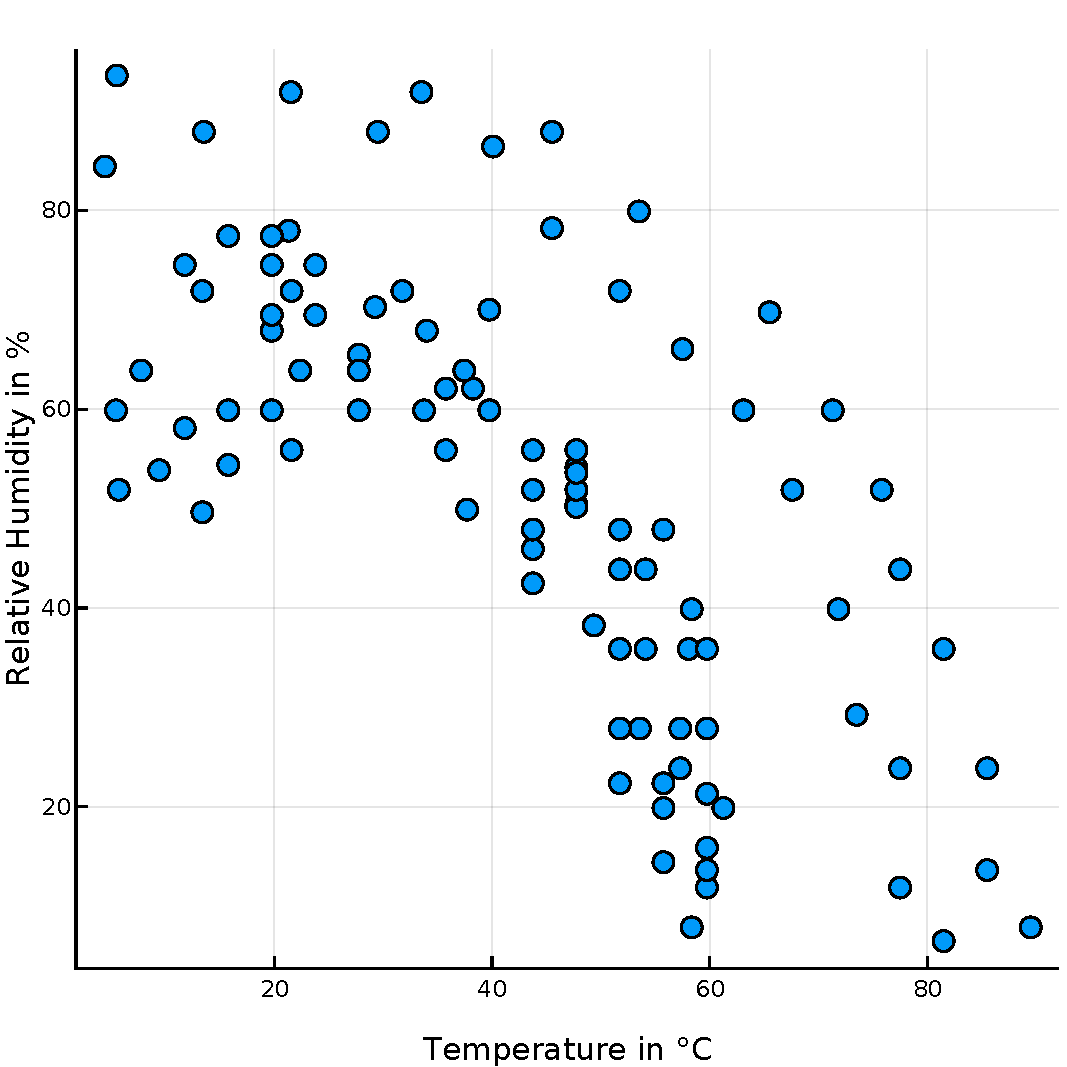
\includegraphics[width=0.33\columnwidth]{clipart/Temperature-initial}

}\subfloat[Count map generated in\protect \\
algorithm step~\ref{enu:AlgoStep3}.]{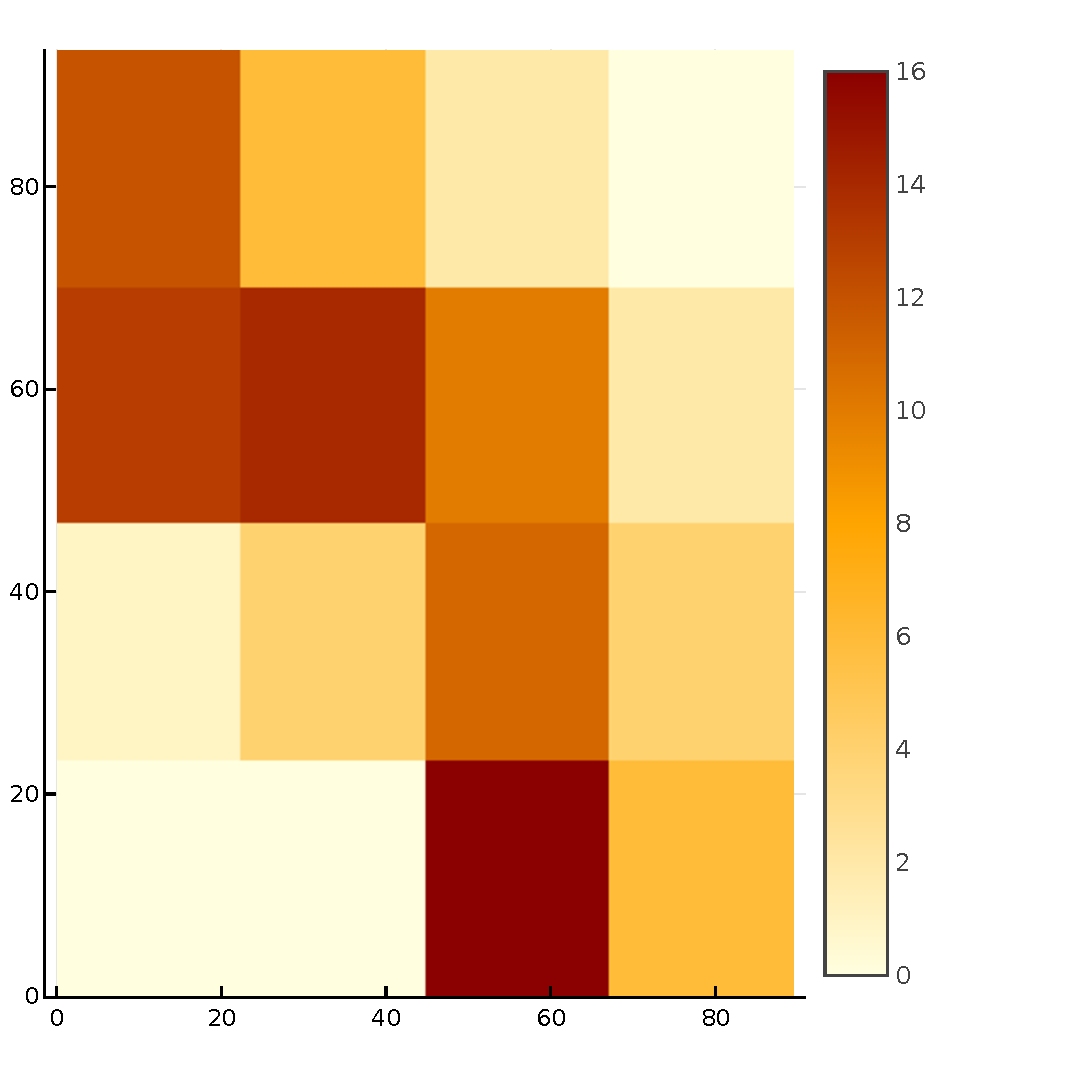
\includegraphics[width=0.33\columnwidth]{clipart/Temperature-4x4-countmap}

}\subfloat[Clustering scheme of the count map.]{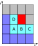
\includegraphics[width=0.29\columnwidth]{clipart/Clustering-Scheme}

}
\par\end{centering}
\caption{\label{fig:Clustering-process}Clustering process of \noun{Iteridense}.
(a) Data to be clustered; (b) Count map generated in of algorithm
step~\ref{enu:AlgoStep3}: 16~cells with the info how many data
points are in.; (c) Clustering scheme of the count map. The red cell
is the currently evaluated cell, the blue cells have already be evaluated,
cells~A\,--\,D are neighboring cells determining the clustering
for the red cell.}
\end{figure}

\begin{enumerate}
\item \label{enu:AlgoStep1}The space of the dataset is divided into a grid
of 4\,\texttimes \,4~cells. In our example the data range of dimension~1
``temperature'' is 4\,--\,89\,�C and the dimension~2 ``humidity''
is 6\,--\,93\,\%. This range defines the space of the dataset.
4\,\texttimes \,4~cells is defined as a resolution of 4. 5\,\texttimes \,5~cells
would be a resolution of 5 and so on.
\item \label{enu:AlgoStep2}The number of data points in the cell spaces
({[}4\,--\,89/4\,�C, 6\,--\,93/4\,\%{]}, {[}89/4\,--\,2�89/4\,�C;
6\,--\,2�93/4\,\%{]}, $\ldots$) are counted. The result is a
count map as shown in \ref{fig:Clustering-process}\,(a).
\item \label{enu:AlgoStep3}Now the actual clustering is performed. The
processing scheme ist depicted in \ref{fig:Clustering-process}\,(b).
Every cell is processed one after another first in x- then in y-direction.
If a cell has more than 1~data point it could be part of a cluster
and then its neighboring cells are evaluated. Thereby only those neighbors
are evaluated that have already be evaluated (blue and light-blue
in \ref{fig:Clustering-process}\,(b)) because for them it is already
known to which cluster they belong to.

If none of the neighbor cells A\,--\,D are in a cluster, the current
cell will start a new cluster. If any neighbor is in a cluster the
current cell will become part of that cluster. If neighbor cells are
in different clusters, these clusters are merged and the current cell
becomes part of that merged cluster. For example cell\,A and cell\,C
could be in different clusters and the current cell unites both clusters.
\item The density of every cluster $\rho_{\mathrm{cluster}}$ is calculated
as the number of points in the cluster divided by the number of cells
in the cluster. To normalize the density, the result is divided by
the density of the whole dataset:
\begin{equation}
\rho_{\mathrm{cluster}}=\cfrac{\text{num points in cluster}}{\text{num cells in cluster}}\cdot\cfrac{\text{total num of cells}}{\text{total num of points}}\label{eq:DensityDefinition}
\end{equation}

So the whole dataset has the density 1.0. As exception, if the clustering
results in a single cluster containing all points, its $\rho_{\mathrm{cluster}}$
is set to 1.0.

The final density $\rho_{\mathrm{final}}$ is the minimum of all $\rho_{\mathrm{cluster}}$.
\item \label{enu:AlgoStep5}All clusters are evaluated. Clusters with $\rho_{\mathrm{cluster}}<1.0$
will be deleted as they are not sensible. Optionally, if $\rho_{\mathrm{cluster}}$
is too low or clusters contain too few data points they are deleted
as well. See the next section of a description of these optional parameters.
The result of this algorithm step is a set of clusters that are subsequently
numbered.
\item The resolution is incremented by one and the steps \ref{enu:AlgoStep1}\,--\,\ref{enu:AlgoStep5}
are repeated until either $\rho_{\mathrm{final}}>\rho$ or until as
many clusters were detected as specified as \textbf{MinClusters}.
To assure that the steps are not repeated forever, the loop is stopped
if the resolution reaches the total number of points in the dataset.
The resolution reached at the end of this step is the final resolution.
\item All data points are assigned according to the found clusters. Points
in cluster ``0'' are hereby not part of a cluster.
\item \label{enu:AlgoStep8}Due to the grid generated in step~\ref{enu:AlgoStep1},
single points might appear in the corner of a cell and are thus not
detected as part of a cluster. Therefore steps \ref{enu:AlgoStep1}\,--\,\ref{enu:AlgoStep5}
are repeated with the final resolution plus 1.
\item Points that were before step~\ref{enu:AlgoStep8} not part of a cluster
but now are, are finally assigned to that cluster. This will only
be done if the number of clusters did not change in step~\ref{enu:AlgoStep8}
and if no data point belongs now to another cluster than before step~\ref{enu:AlgoStep8}.
\end{enumerate}
\ref{fig:Result-Iteridense} shows the result for $\rho=3.0$. The
final resolution is 13, there is one cluster with $\rho_{\mathrm{cluster}}=4.32$.

\begin{figure}
\begin{centering}
\hfill{}\subfloat[Resulting data point assignment.]{\begin{centering}
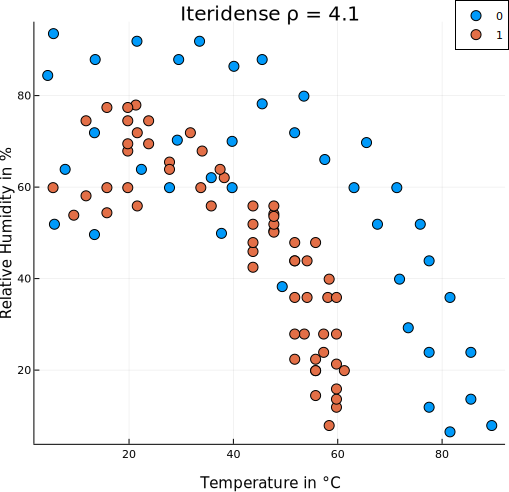
\includegraphics[scale=0.4]{clipart/Temperature-final}
\par\end{centering}
}\hfill{}\subfloat[Final count map (resolution 13).]{\begin{centering}
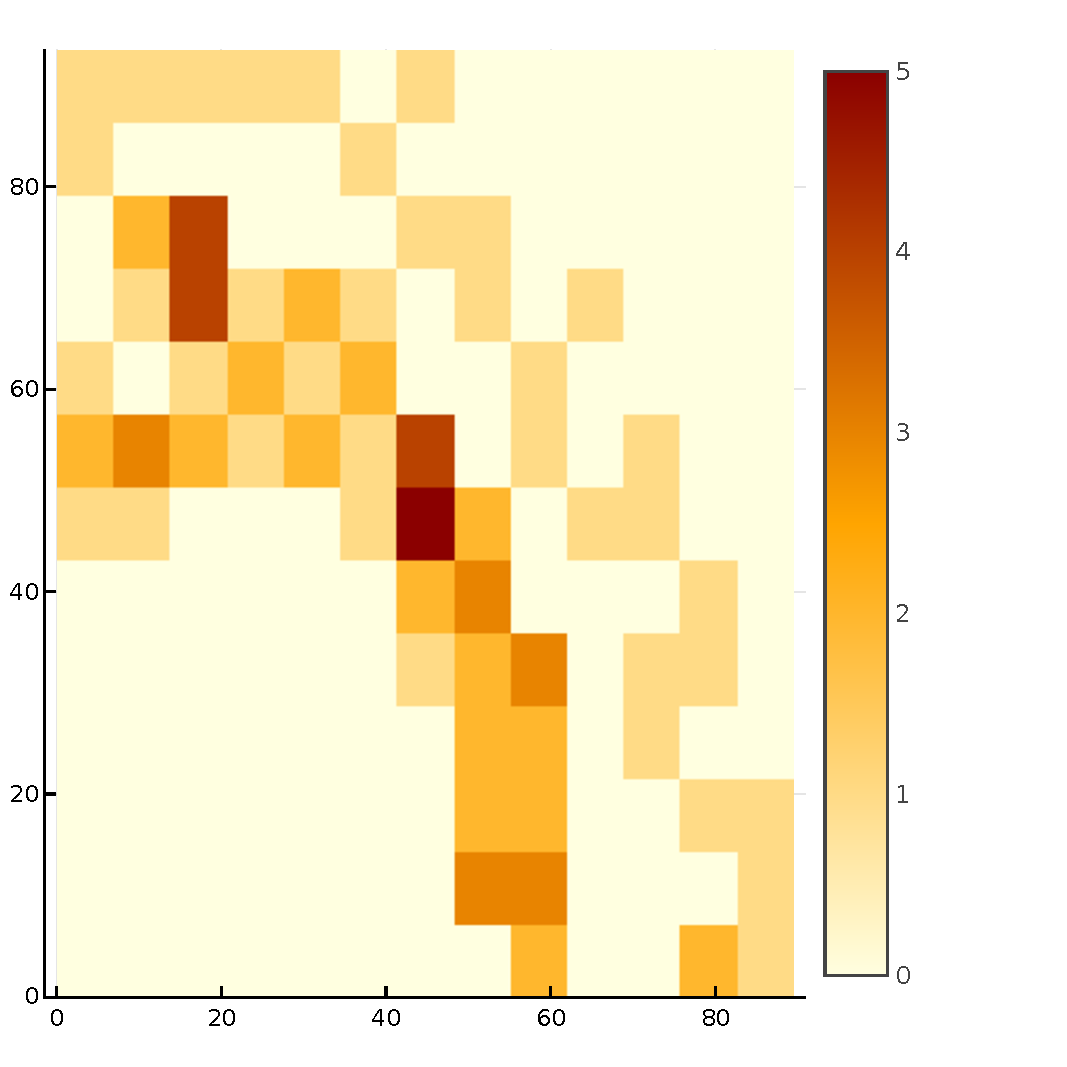
\includegraphics[scale=0.4]{clipart/Temperature-13x13-countmap}
\par\end{centering}
}\hfill{}
\par\end{centering}
\caption{\label{fig:Result-Iteridense}Result of \noun{Iteridense} for the
dataset in \ref{fig:Data-the-2dimensions} for $\rho=3.0$.}
\end{figure}


\subsection{Options}

The algorithm can optionally be modified this way:
\begin{enumerate}
\item \label{enu:Specification-of-the}Specification of the start resolution
for step~\ref{enu:AlgoStep1} (\textbf{StartResolution}). The default
and minimum is 2, the maximum is the total number of points in the
dataset.
\item \label{enu:OptionDiagonal}In step~\ref{enu:AlgoStep3} don't take
cells into account that are diagonally connected to the current cell
(\textbf{NoDiagonals}). In \ref{fig:Clustering-process}\,(b) cells~A
and C would then not be evaluated.
\item \label{enu:OptionClusterSize}Specification of the minimal number
of data points in a cluster (\textbf{MinClusterSize}). Clusters with
less points will be erased. The default is 3, the minimum is 2, the
maximum is the total number of points in the dataset minus 1.
\item \label{enu:OptionClusterDensity}Specification of the minimal $\rho_{\mathrm{cluster}}$
of a cluster (\textbf{MinClusterDensity}). Clusters with lower $\rho_{\mathrm{cluster}}$
will be erased. The minimum and default is 1.0.
\item \label{enu:Specification-of-a}Specification of a resolution at which
the loop step~\ref{enu:AlgoStep1}\,--\,\ref{enu:AlgoStep5} is
stopped\\
 (\textbf{StopResolution}).
\item \label{enu:OptionFixedResolution}Instead of a the loop step~\ref{enu:AlgoStep1}\,--\,\ref{enu:AlgoStep5},
run the steps once with a fixed resolution\linebreak{}
 (\textbf{FixedResolution}).
\end{enumerate}
Option~\ref{enu:Specification-of-the} can speed up the computation
significantly.

Option~\ref{enu:OptionDiagonal} can be useful for a low $\rho$
(and thus low resolutions)\footnote{For example with \textbf{NoDiagonals} in \ref{fig:Result-Iteridense}
with $\rho=2.2$ the cluster would contain more points.} while for higher $\rho$ and also high dimensions it might lead to
bad results. Therefore this option should only be used if really desired.

Option~\ref{enu:OptionClusterSize} is useful to exclude unsuitably
small clusters. It is recommended to set $\text{\textbf{MinClusterSize}}\ge D+1$
where $D$ is the dimensionality of the data set.

Option~\ref{enu:OptionClusterDensity} has only an effect if \textbf{MinClusters}
is used. It helps to sort out clusters with a density too low to be
sensible for the use case.

Option~\ref{enu:Specification-of-a} prevents undesired many loops.
For example if $\rho$ was set to a high value and no cluster will
be found.

Option~\ref{enu:OptionFixedResolution} is only useful for academic
purpose. However, it is internally used for step~\ref{enu:AlgoStep8}.

A reference implementation of \noun{Iteridense} is online available~\cite{Iteridense}.
Its outputs are besides the assignments of the points to clusters
also the size of clusters, density of clusters, final resolution,
number of clusters, the count map as tensor in the final resolution
(the actual probability-density function) and a tensor like the count
map but with information about what cluster a grid cell belongs to.

\section{Clustering Results}

To show the clustering results artificial data was generated using
the library \emph{sklearn.datasets} from the scikit-learn project~\cite{SciKitLearnDataSets}.
Real data were taken from the \emph{Rdatasets} database~\cite{Rdatasets}.
All clustering results figures were created using the package \emph{Plots}
of the \noun{Julia} programming language~\cite{JuliaPlots}.

\subsection{Effect of the Density Parameter}

The data shown in \ref{fig:Result-of-the} and \ref{fig:Effect-of-a}
was generated using the \emph{make\_moons }call to \emph{sklearn.datasets}.
\ref{fig:Result-of-the}\,(a) shows the result for $\rho=2.2$, \ref{fig:Result-of-the}\,(b)
shows the result for $\rho=5.0$. As derived in \ref{sec:Derivation-of-the},
the greater the density means, translated to the relief example, the
area of the cluster gets smaller. Therefore less points are assigned
to the clusters for $\rho=5.0$.

\begin{figure}[h]
\begin{centering}
\hfill{}\subfloat[$\rho=2.2$, resulting resolution: 12]{\begin{centering}
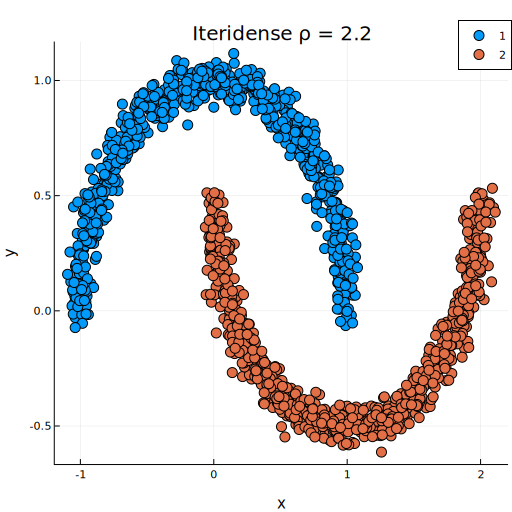
\includegraphics[scale=0.4]{clipart/Moons-Iteridense-rho2-2}
\par\end{centering}
}\hfill{}\subfloat[$\rho=5.0$, resulting resolution: 43]{\begin{centering}
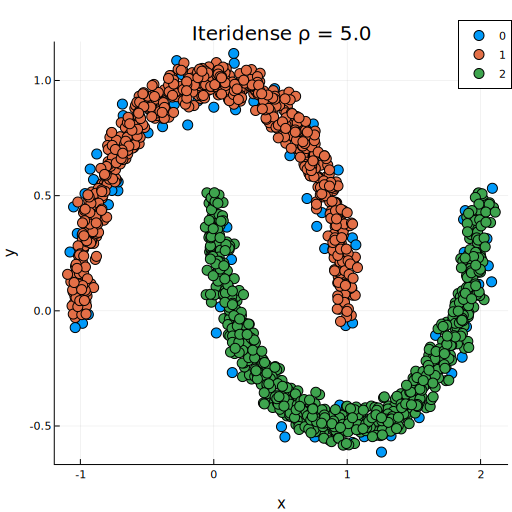
\includegraphics[scale=0.4]{clipart/Moons-Iteridense-rho5}
\par\end{centering}
}\hfill{}
\par\end{centering}
\caption{\label{fig:Result-of-the}Result of \noun{Iteridense} for intersected
moon-like clusters using different $\rho$.}
\end{figure}

\ref{fig:Effect-of-a} shows the result for $\rho=6.0$. The density
is now so high that the moon-like clusters break down into many small
clusters if the option \textbf{NoDiagonals} is used for the clustering.

\begin{figure}
\begin{centering}
\hfill{}\subfloat[$\rho=6.0$ with option \textbf{NoDiagonals}, resulting resolution:
68]{\begin{centering}
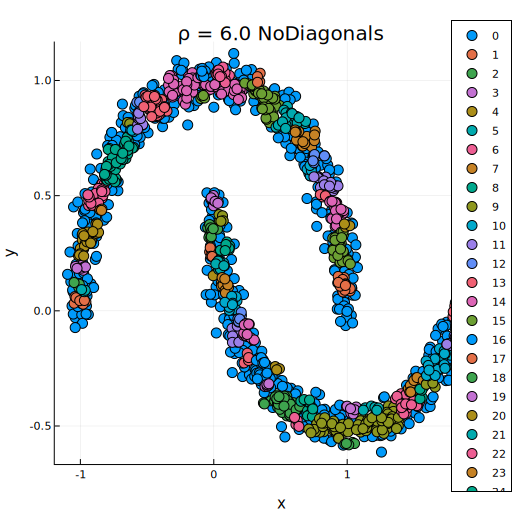
\includegraphics[scale=0.4]{clipart/Moons-Iteridense-rho6-noDiagonals}
\par\end{centering}
}\hfill{}\subfloat[$\rho=6.0$, resulting resolution: 52]{\begin{centering}
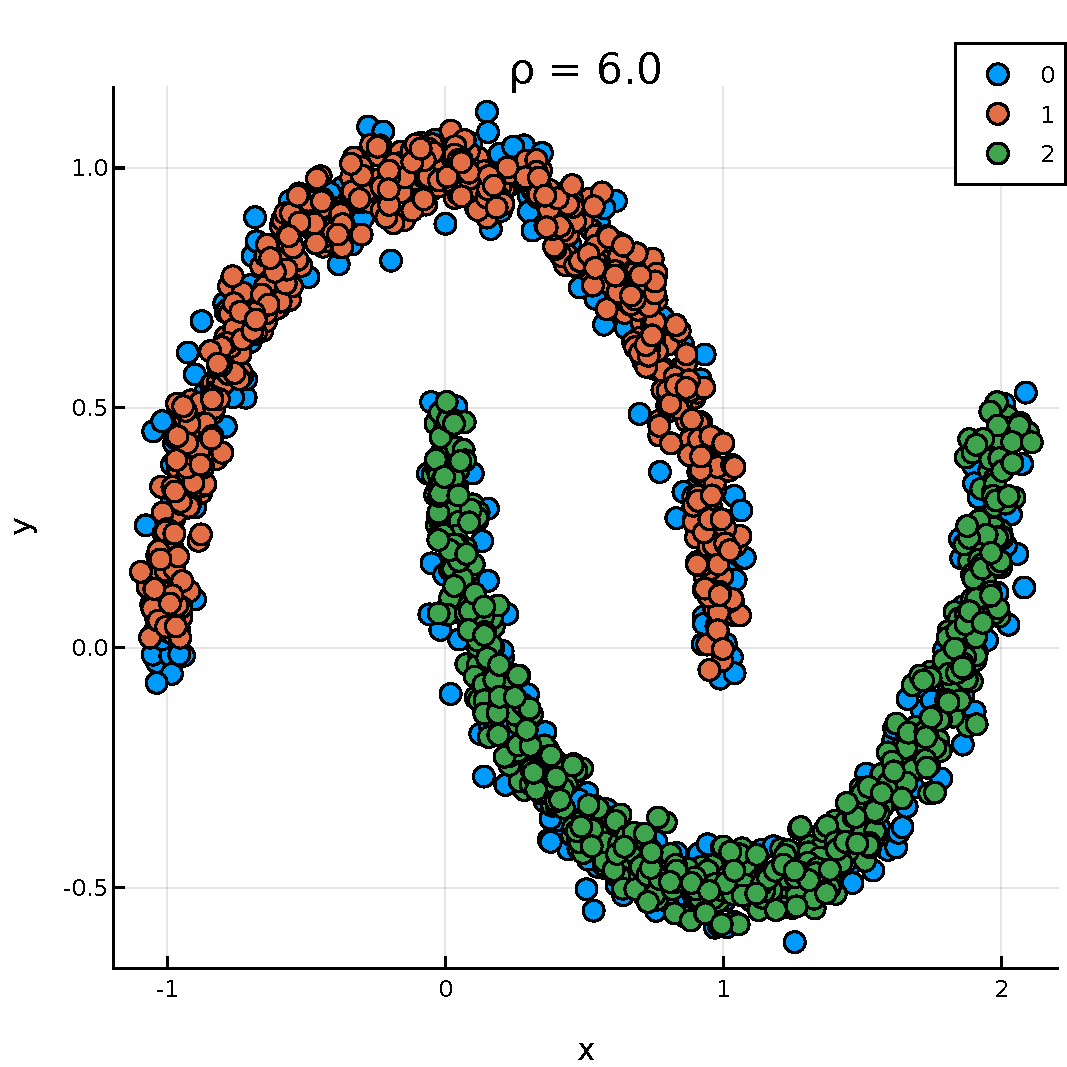
\includegraphics[scale=0.4]{clipart/Moons-Iteridense-rho6}
\par\end{centering}
}\hfill{}
\par\end{centering}
\caption{\label{fig:Effect-of-a}Effect of a high $\rho$ and the option to
evaluate neighbor cells on the clustering result.}
\end{figure}


\subsection{Clustering Performance\label{subsec:Clustering-Performance}}

An advantage compared to other clustering algorithm is that \noun{Iteridense}
treats all data points the same way. There is no division between
core points, outliers or the like. Another major feature of \noun{Iteridense}
is that it provides two ways to achieve results and a clear path for
the user on how to change the input parameters to get a suitable result:\pagebreak{}
\begin{itemize}
\item Either start with a low $\rho$ and increase it gradually to get a
suitable result. If the result is not suitable, look at the resulting
$\rho_{\mathrm{cluster}}$ and set for the next run $\rho$ above
their minimum.
\item Or specify with \textbf{MinClusters} the desired number of clusters.
If the result is not suitable, increase gradually either \textbf{MinClusterSize}
or \textbf{MinClusterDensity}.
\end{itemize}
The second path is computationally the fastest, as discussed in the
next section. However, it can only be taken if there is a physical
or technical reason for the number of clusters. For the path to specify
$\rho$ \ref{fig:Result-Iteridense-Blobs}\,(a)\,--\,\ref{fig:Result-Iteridense-Blobs2}\,(a)
shows the results: Until $\rho\le6.8$ only one cluster is detected
and starting at $\rho=7.3$ there are 3~clusters. Increasing $\rho$
leads to more and more clusters. This can be used to identify regions
with higher density inside a ``base'' cluster. In the example there
are 3~base clusters and every one has more dense regions that are
unveiled with greater $\rho$.

\begin{figure}[p]
\begin{centering}
\hfill{}\subfloat[$\rho=6.8$, resulting resolution: 30]{\begin{centering}
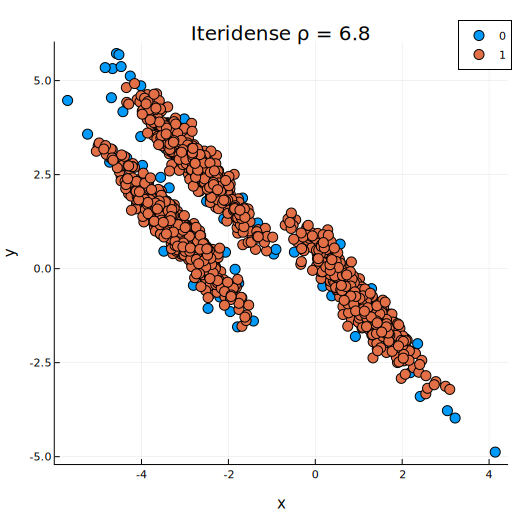
\includegraphics[scale=0.4]{clipart/Anisotropes-Iteridense-rho6-8}
\par\end{centering}
}\hfill{}\subfloat[$\rho=7.3$, resulting resolution: 35]{\begin{centering}
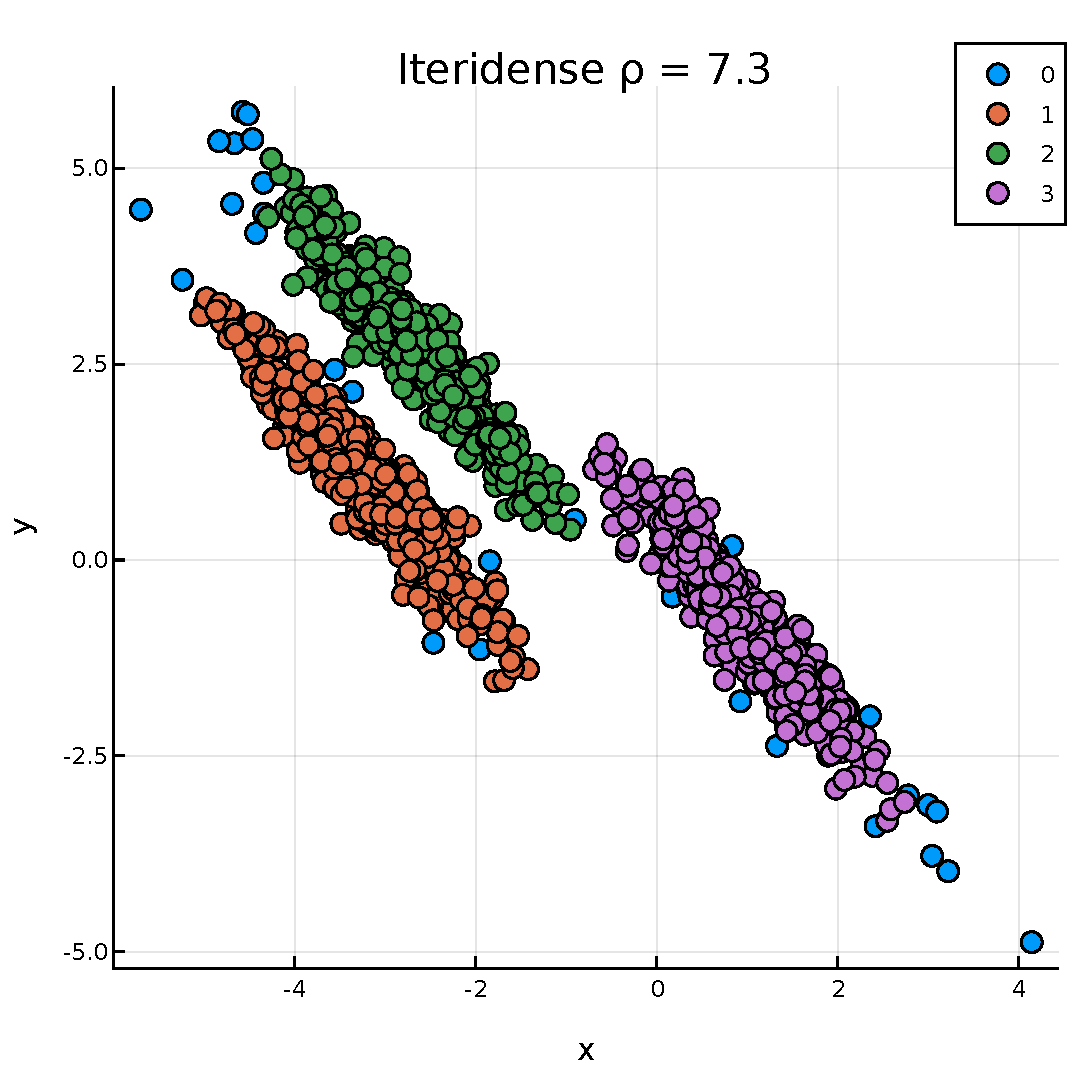
\includegraphics[scale=0.4]{clipart/Anisotropes-Iteridense-rho7-3}
\par\end{centering}
}\hfill{}
\par\end{centering}
\caption{\label{fig:Result-Iteridense-Blobs}Result of \noun{Iteridense} for
$\rho\ge7.3$ \textbf{MinClusterSize~=~}6 at anistotope clusters.}
\end{figure}

\begin{figure}[p]
\begin{centering}
\hfill{}\subfloat[$\rho=12.0$, resulting resolution: 84]{\begin{centering}
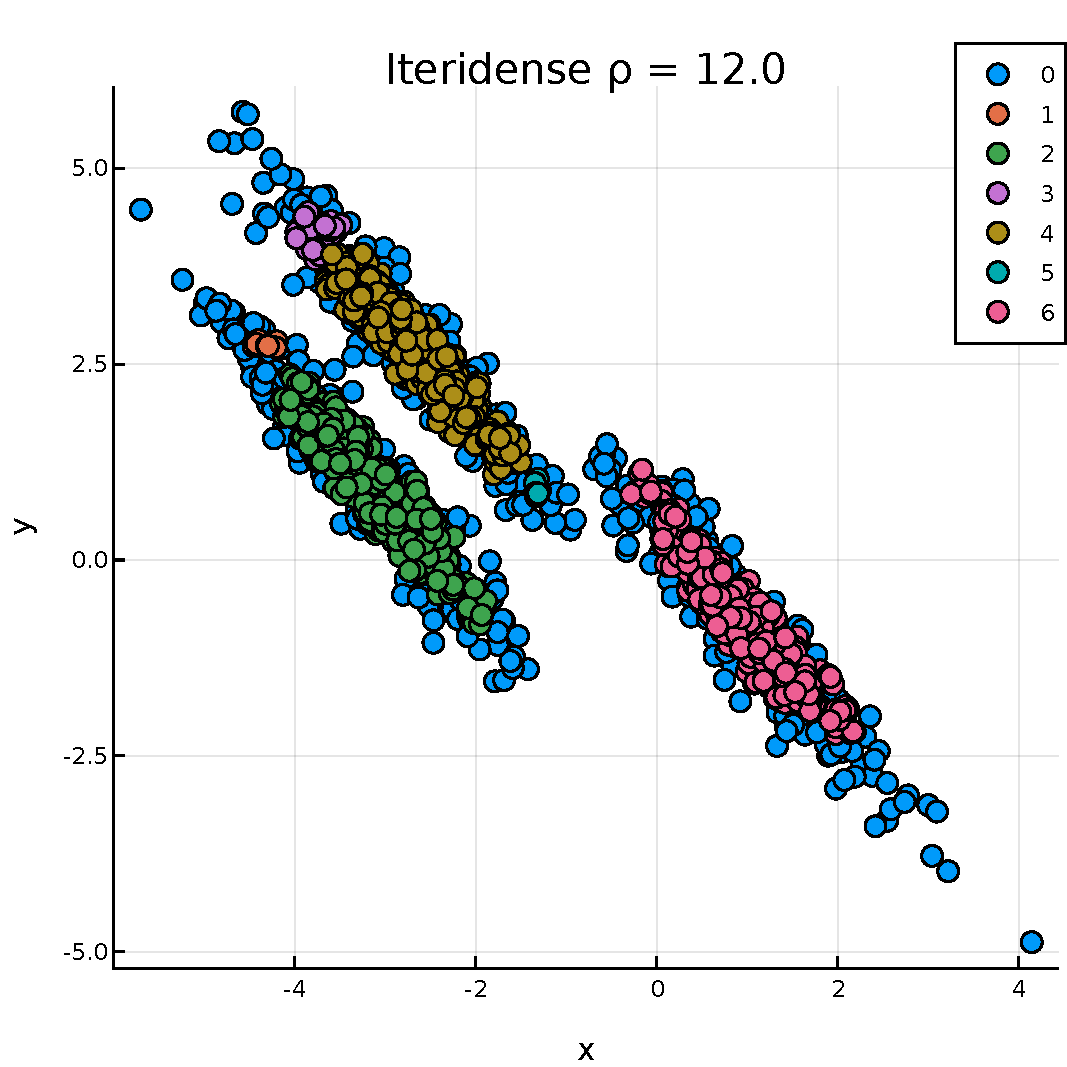
\includegraphics[scale=0.4]{clipart/Anisotropes-Iteridense-rho12}
\par\end{centering}
}\hfill{}\subfloat[$\epsilon=0.1$]{\begin{centering}
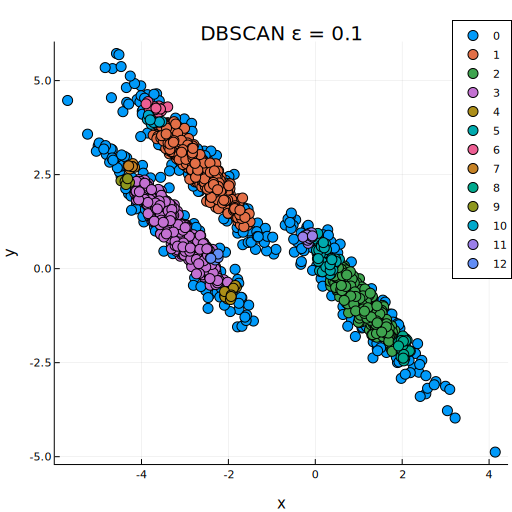
\includegraphics[scale=0.4]{clipart/Anisotropes-DBSCAN-eps0-10}
\par\end{centering}
}\hfill{}
\par\end{centering}
\caption{\label{fig:Result-Iteridense-Blobs2}Result of \noun{Iteridense} for
$\rho=6.8$ and DBSCAN for $\epsilon=0.1$ at anistotope clusters.}
\end{figure}

For comparison, the algorithm DBSCAN does not provide a clear path
on how to change its input parameters. An example is the data shown
in \ref{fig:Result-Iteridense-Blobs2}\,(b). This data was generated
using the \emph{make\_blobs }call to \emph{sklearn.datasets} with
a subsequent transformation. Like in the previous example, there are
1500~data points.

$\epsilon=0.1$ seems to be a sensible start value for DBSCAN. The
result is \ref{fig:Result-of-DBSCAN}\,(b). As the result is not
a useful one might increase $\epsilon$ in small steps and gets with
\textbf{MinPts} (minimal points to form a dense region) of 6 as results
\ref{fig:Result-of-DBSCAN}\,--\,\ref{fig:Result-of-DBSCAN-1}.
For this dataset a human would expect 3~base clusters but DBSCAN
does not find exactly 3~clusters. One has to try different $\epsilon$
to get this result. For data in 2 or 3~dimensions one can plot the
data to get a feeling for $\epsilon$ and for example increase \textbf{MinPts}.
However, for data in higher dimensions this is hardly possible.

\begin{figure}[p]
\begin{centering}
\hfill{}\subfloat[$\epsilon=0.15$]{\begin{centering}
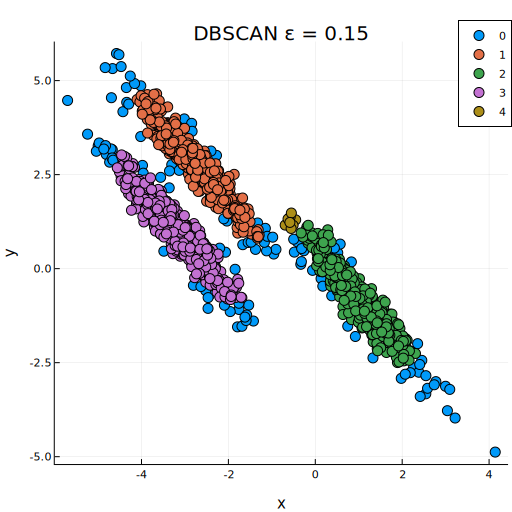
\includegraphics[scale=0.4]{clipart/Anisotropes-DBSCAN-eps0-15}
\par\end{centering}
}\hfill{}\subfloat[$\epsilon=0.2$]{\begin{centering}
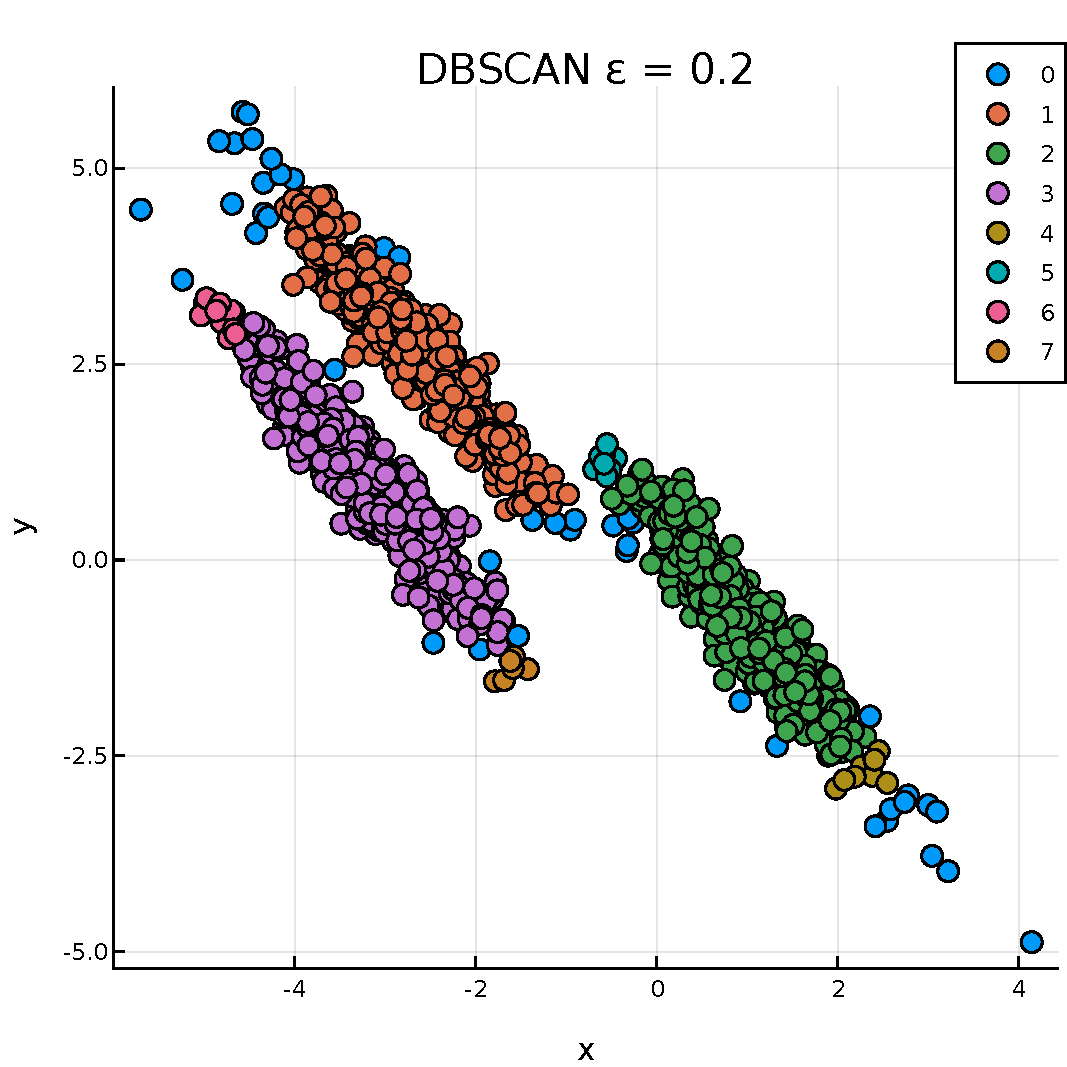
\includegraphics[scale=0.4]{clipart/Anisotropes-DBSCAN-eps0-20}
\par\end{centering}
}\hfill{}
\par\end{centering}
\caption{\label{fig:Result-of-DBSCAN}Result of DBSCAN at anistotope clusters
with $\epsilon\le0.2$.}
\end{figure}

\begin{figure}[p]
\begin{centering}
\hfill{}\subfloat[$\epsilon=0.25$]{\begin{centering}
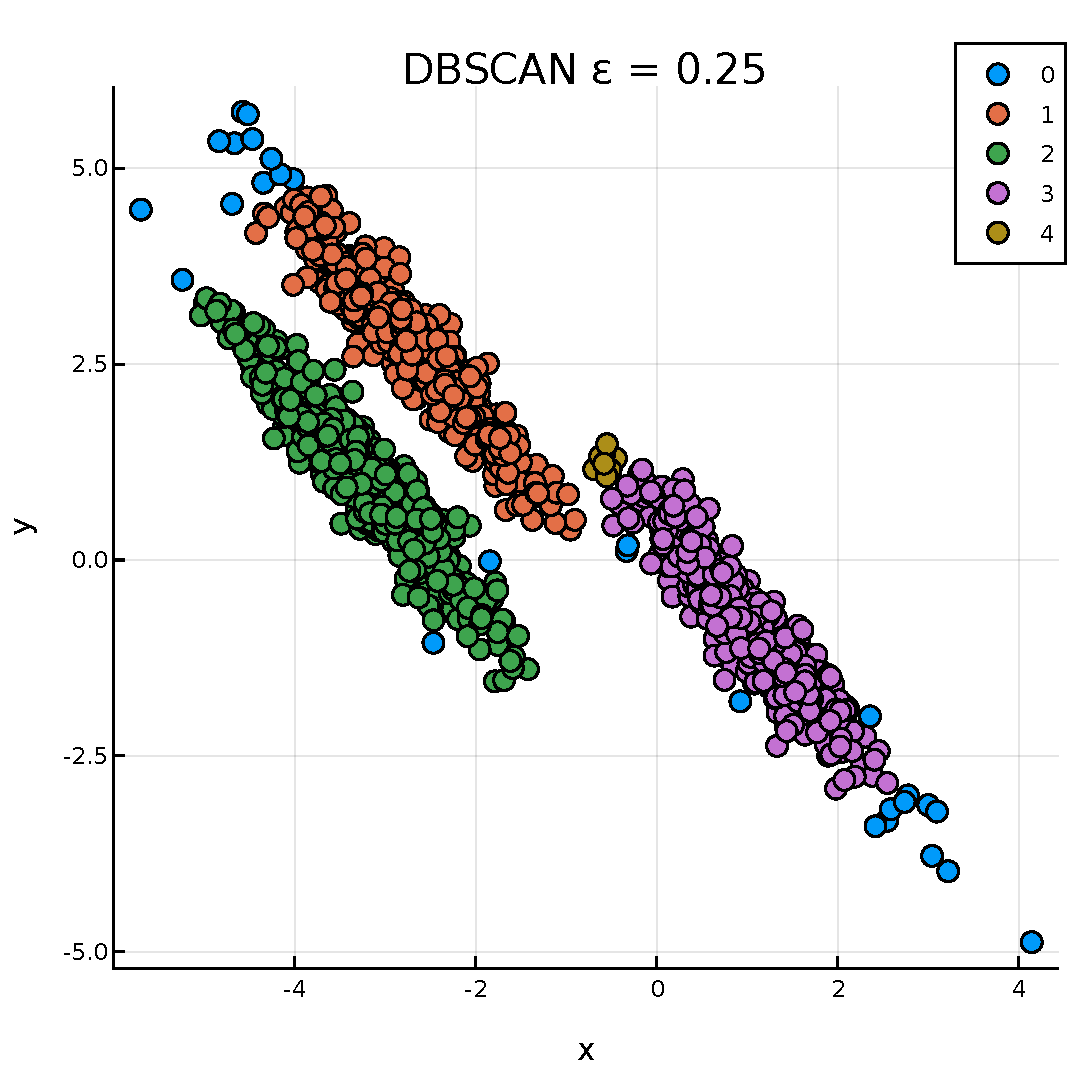
\includegraphics[scale=0.4]{clipart/Anisotropes-DBSCAN-eps0-25}
\par\end{centering}
}\hfill{}\subfloat[$\epsilon=0.3$]{\begin{centering}
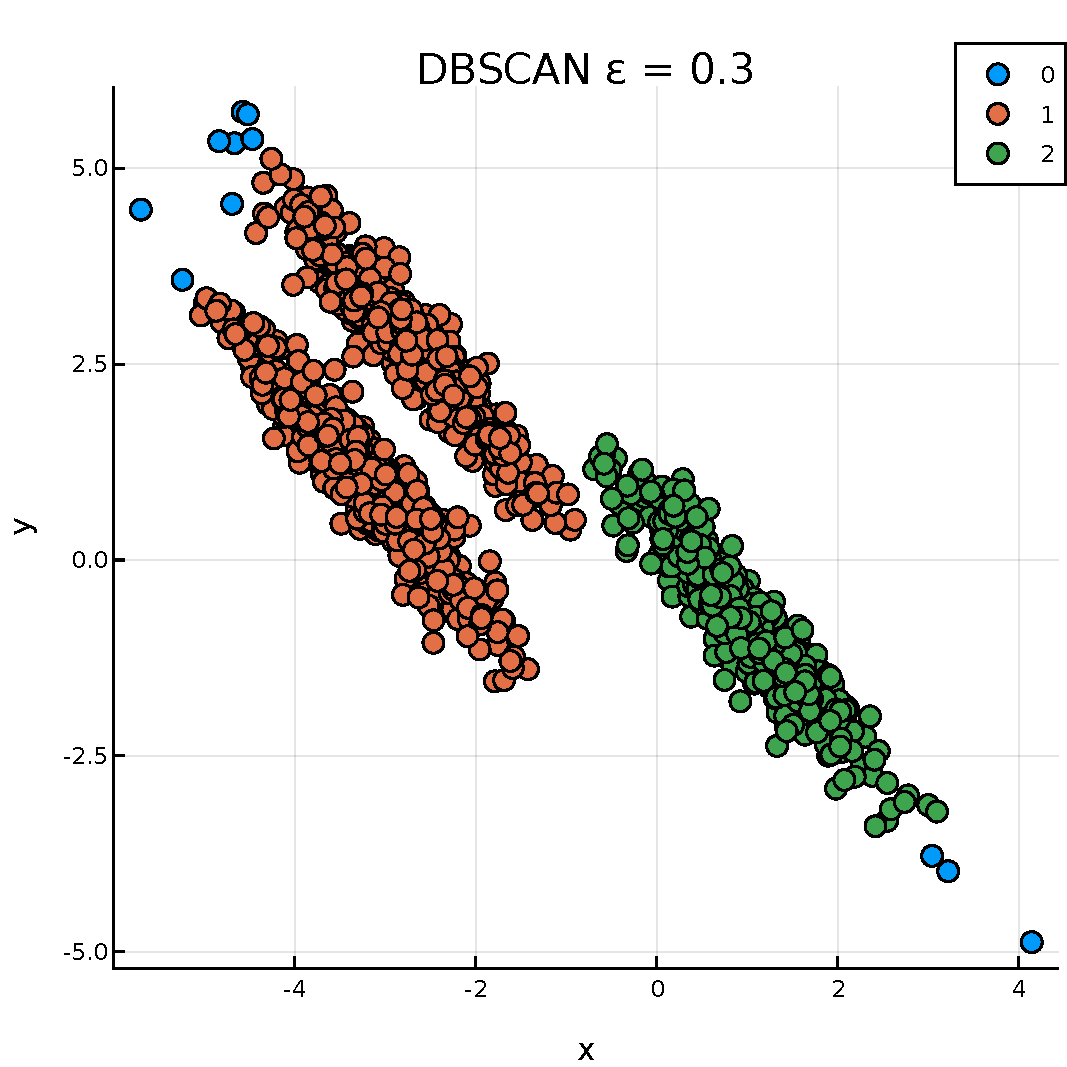
\includegraphics[scale=0.4]{clipart/Anisotropes-DBSCAN-eps0-30}
\par\end{centering}
}\hfill{}
\par\end{centering}
\caption{\label{fig:Result-of-DBSCAN-1}Result of DBSCAN at anistotope clusters
with $\epsilon>0.2$.}
\end{figure}

\ref{fig:Result-of-Iteridense-NoisyBlobs}\,(a) is another example
with 1500~data points, generated using the \emph{make\_blobs }call
to \emph{sklearn.datasets} with a subsequent transformation. \textbf{MinClusters}
was set to 2 and \textbf{MinClusterSize} 20. Cluster~2 has $\rho_{\mathrm{cluster}}=3.07$
and is a merge of a high- and low-density region. The two ways to
change or to achieve a certain result are:\pagebreak{}
\begin{itemize}
\item Either set \textbf{MinClusters} to 3 to get two clusters with a high
density and one with a lower density, see \ref{fig:Result-of-Iteridense-NoisyBlobs}\,(b).
\item Or increase $\rho$ and also increase \textbf{MinClusterSize} e.g.~to
50 unless one gets only 2~high-density clusters, see \ref{fig:Result-of-Iteridense-NoisyBlobs}\,(c).
Increasing \textbf{MinClusterSize} is hereby necessary to avoid small
clusters in the low-density area.
\end{itemize}
The change of \textbf{MinClusterSize} might not be obvious when one
cannot plot for example high-dimensional data. But that this is the
way to go is a feature of the the \noun{Iteridense} algorithm.

\begin{figure}
\begin{centering}
\subfloat[\textbf{MinClusters} = 2]{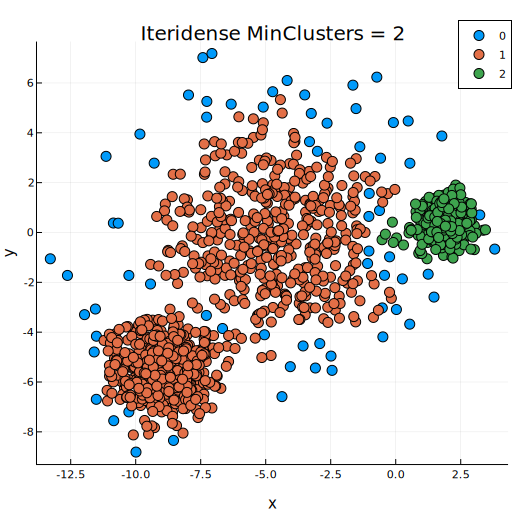
\includegraphics[width=0.33\columnwidth]{clipart/BlobNoise-Iteridense-MinClusters2}

}\subfloat[\textbf{MinClusters} = 3]{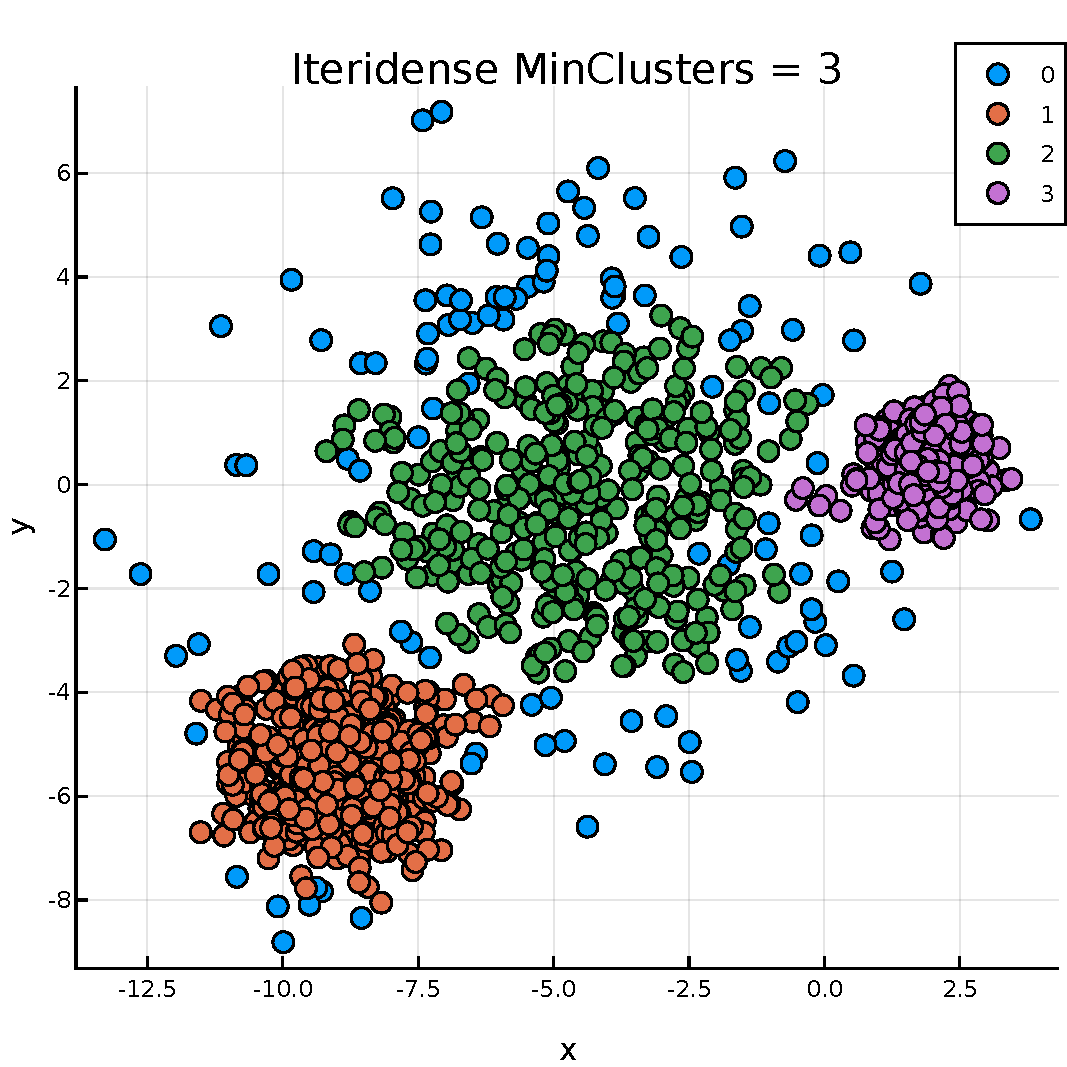
\includegraphics[width=0.33\columnwidth]{clipart/BlobNoise-Iteridense-MinClusters3}

}\subfloat[$\rho=4.3$,\protect \\
\textbf{MinClusterSize} = 50]{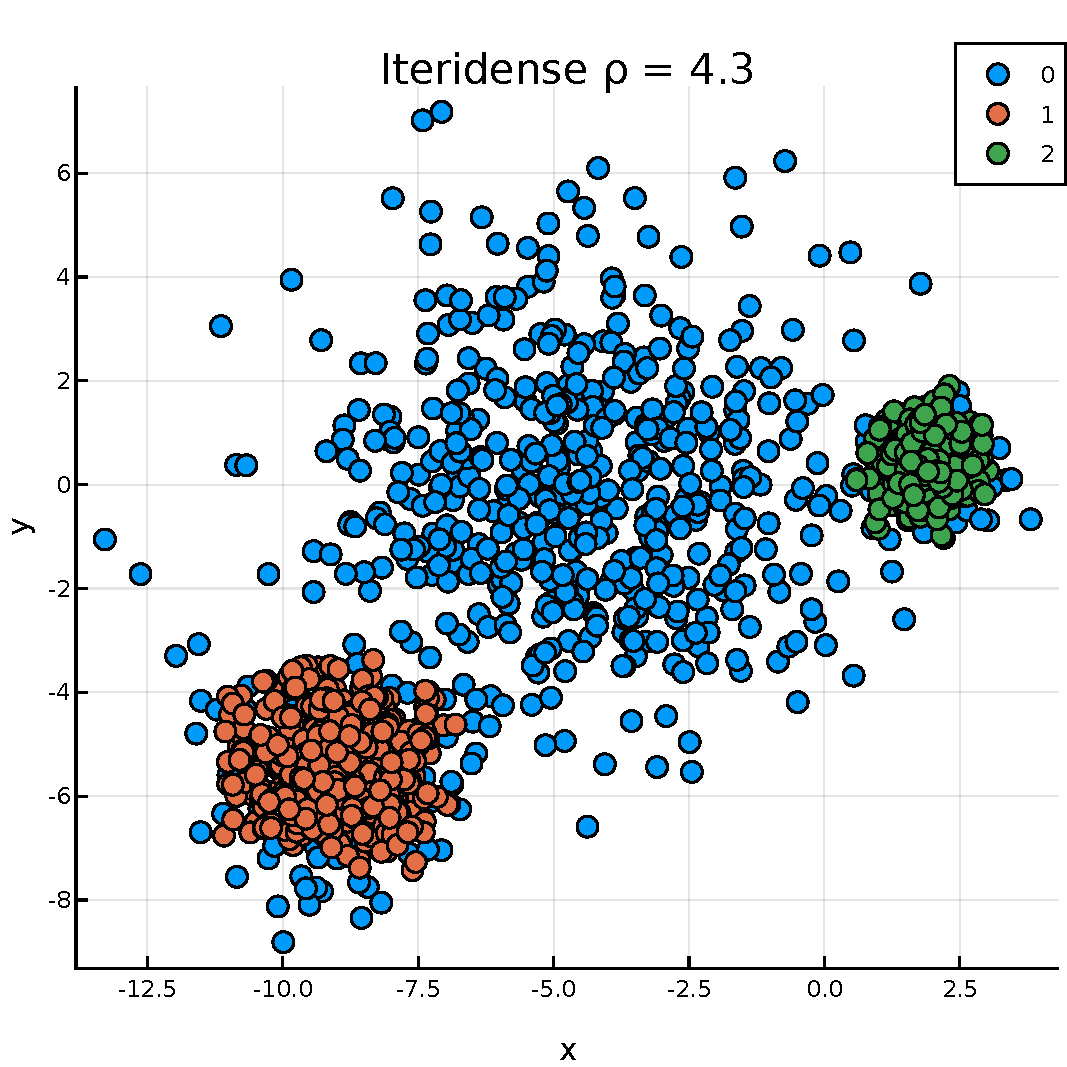
\includegraphics[width=0.33\columnwidth]{clipart/BlobNoise-Iteridense-rho4-3}

}
\par\end{centering}
\caption{\label{fig:Result-of-Iteridense-NoisyBlobs}Result of \noun{Iteridense}
for clusters with different densities.}
\end{figure}


\subsection{Computation Performance}

The data shown in \ref{fig:Result-Iteridense-Circles} was generated
using the \emph{make\_circles }call to \emph{sklearn.datasets}.

In that case, there must be 2~clusters, therefore one can specify
\textbf{MinClusters}. This will lead to a shorter computation as with
the specification of $\rho$ since the algorithm loop is stopped as
soon as 2~clusters are detected, otherwise there might be further
loops. For our example 10,000~cluster runs with \textbf{MinClusters~}=~2
took $\approx9.4\thinspace$s\footnote{The times were measured using the feature \emph{@elapsed} of the \noun{Julia}
programming language.} and the final resolution was 13. For $\rho=2.0$ the final resolution
was 25 and with $\approx24\thinspace$s more time was needed. By starting
the algorithm at a higher resolution, e.\,g. with \textbf{StartResolution~}=~10
the time would decrease from $\approx9.4\thinspace$s to $\approx7.1\thinspace$s.

\ref{fig:Result-Iteridense-Circles}\,(a) shows the \noun{Iteridense}
result. For comparison \ref{fig:Result-Iteridense-Circles}\,(b)
shows the result using the DBSCAN algorithm for $\epsilon=0.1$ and
$\text{\textbf{MinPts}}=3$.

The benefit of \noun{Iteridense} compared to density-based algorithms
is the computation time. In this example the dataset has 1500~data
points. To generate the count map in algorithm step~\ref{enu:AlgoStep1},
every data point has to be evaluated in form of generating its coordinate
value for the current grid coordinate system. This is the most costly
operation, especially for high-dimensional data. Afterwards, only
the cells have to be evaluated, not the data points. For DBSCAN in
comparison the coordinates for every data point are only read out
once but the distances between every point and neighboring points
have to be calculated. The larger $\epsilon$ or the greater the point
density the more points are neighbors and have to be evaluated. This
can become very computation-intensive. For the data of \ref{fig:Result-Iteridense-Circles}
with $\epsilon=0.1$ and $\text{\textbf{MinPts}}=3$ 10,000~cluster
runs took $\approx17.8\thinspace$s while the same with $\epsilon=0.5$
took $\approx69\thinspace$s and with $\epsilon=0.5$ both clusters
were even not detected.\footnote{The computation time measurement of the DBSCAN algorithm was performed
using its implementation in the package \emph{Clustering} of the \noun{Julia}
programming language~\cite{ClusteringDBSCAN}.} Therefore setting $\epsilon$ to a suitable value does not only affect
the result a lot but also the computation time. Since there is no
clear path on how to change $\epsilon$ to get a useful result, more
cluster runs have to be performed than with \noun{Iteridense}.

For \noun{Iteridense} the worst case in terms of computation is to
set $\rho$ so high that the algorithm runs 1500\,loops as there
are 1500~data points. A single run of this takes $\approx13.4\thinspace$s.
So 1500\,loops take longer than 10.000~times the 12~loops from
the default \textbf{StartResolution} 2 to the final resolution~13.
This is because the number of cells in the grid scales in 2~dimensions
squarely with the resolution. To prevent that undesired many loops
are run, the parameter \textbf{StopResolution} can be set.

\begin{figure}
\begin{centering}
\hfill{}\subfloat[\textbf{MinClusters} = 2, resulting resolution: 16]{\begin{centering}
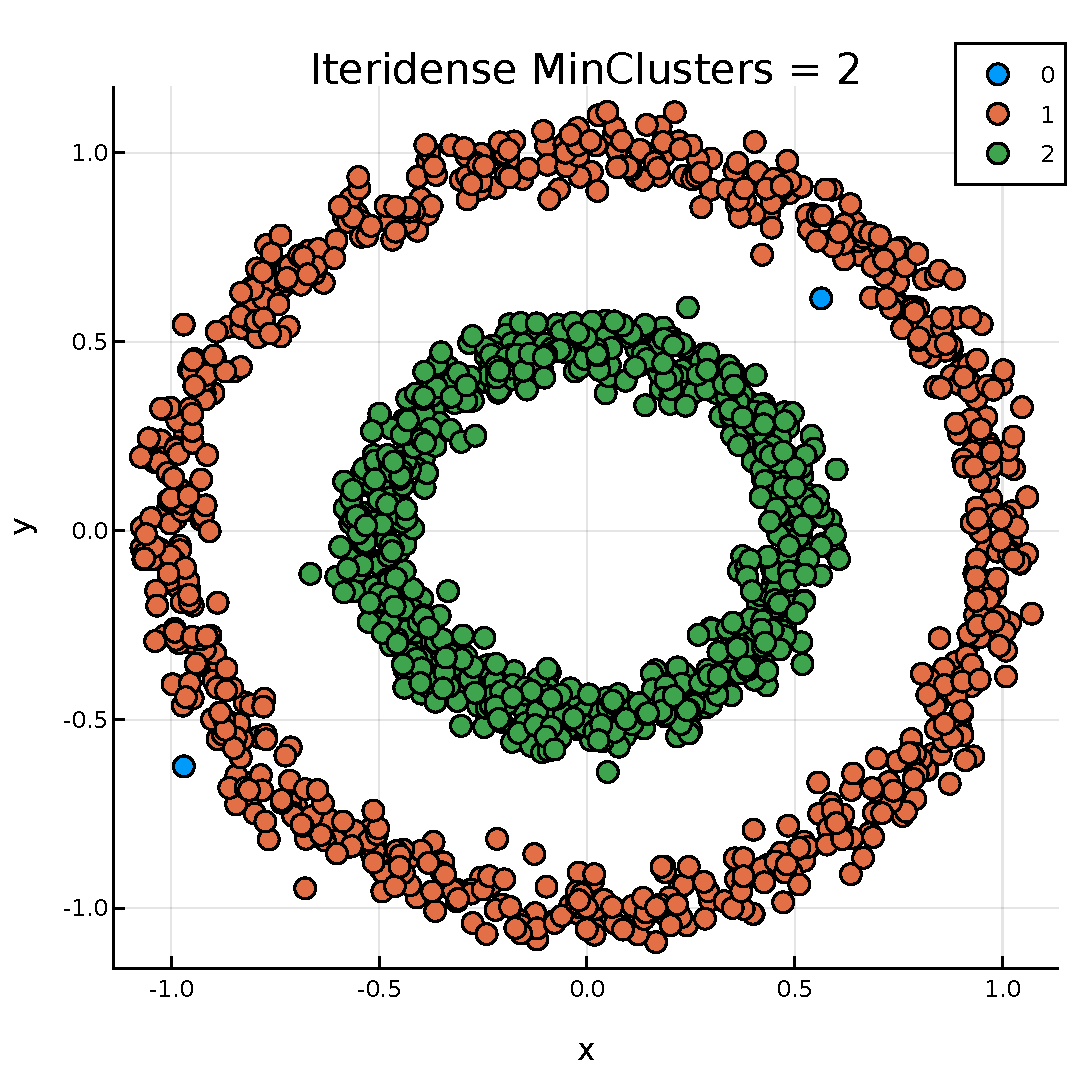
\includegraphics[scale=0.4]{clipart/Circles-Iteridense-MinClusters2}
\par\end{centering}
}\hfill{}\subfloat[$\epsilon=0.1$]{\begin{centering}
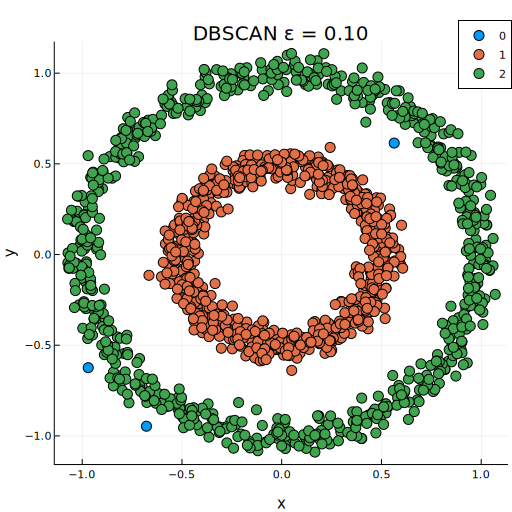
\includegraphics[scale=0.4]{clipart/Circles-DBSCAN-eps0-1}
\par\end{centering}
}\hfill{}
\par\end{centering}
\caption{\label{fig:Result-Iteridense-Circles}Result of \noun{Iteridense}
and DBSCAN for intersected circle-like clusters.}
\end{figure}


\subsection{Results in higher Dimensions}

Data with higher dimensions are a main use case for clustering algorithms
as no human could do the clustering according to plots. \ref{fig:Iteridense-Pluton}
is an example and also demonstrate the clustering performance of \noun{Iteridense}.
The data are the publicly available \emph{pluton} dataset\cite{RDataPluton}
containing concentrations of the different Plutonium isotopes in 45~ore
samples. It has 4~dimensions.

\begin{figure}
\begin{centering}
\subfloat[Clustering with only shown\protect \\
dimensions taken into account.]{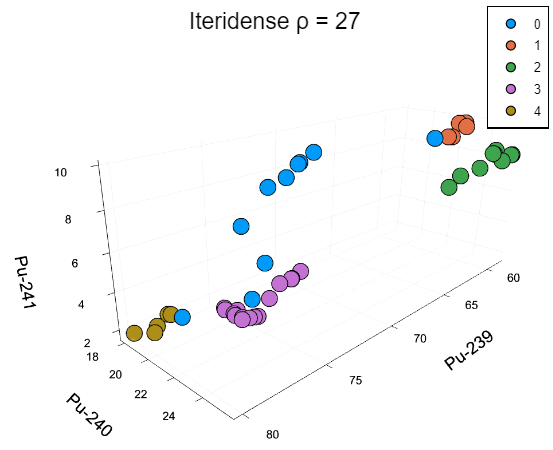
\includegraphics[width=0.33\columnwidth]{clipart/Pluto-Iteridense-rho27-only3}

}\subfloat[Clustering with all dimensions taken into account.]{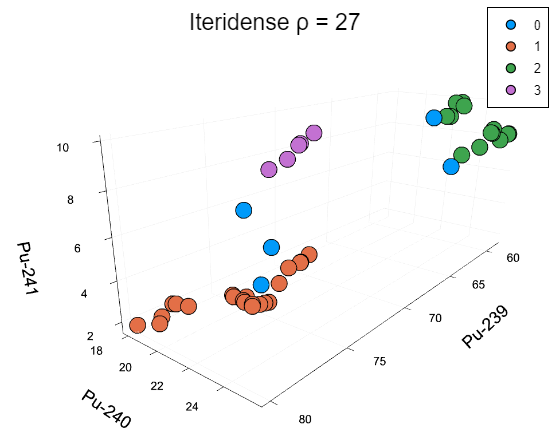
\includegraphics[width=0.33\columnwidth]{clipart/Pluto-Iteridense-rho27-all}

}\subfloat[like (b) but $\rho=106$]{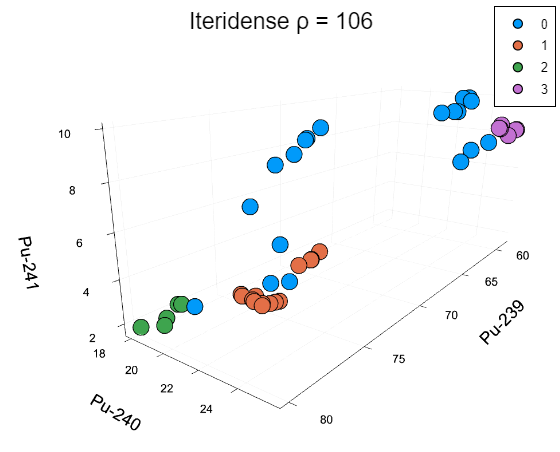
\includegraphics[width=0.33\columnwidth]{clipart/Pluto-Iteridense-rho106-all}

}
\par\end{centering}
\caption{\label{fig:Iteridense-Pluton}Result of \noun{Iteridense} for the
\emph{pluton} dataset.}
\end{figure}

By plotting 3~dimensions of the dataset and performing \noun{Iteridense}
only on the plotted dimensions, the result would be \ref{fig:Iteridense-Pluton}\,(a).
Taking all dimensions into account, the result is \ref{fig:Iteridense-Pluton}\,(b).
The points of high Pu-241 concentrations are then identified as a
cluster. Cluster~1 is so large because its density in all 4~dimensions
matters. If one wants for some reason cluster~1 to be split into
2~clusters, one follows the \noun{Iteridense} path and increases
$\rho$ above the lowest $\rho_{\mathrm{cluster}}$and ends up with
\ref{fig:Iteridense-Pluton}\,(c). The high value for $\rho$ is
the result of the high dimensionality of the data.\\
For comparison DBSCAN cannot find in this dataset more than 2~clusters.

\ref{fig:Result-Iteridense-PhD} shows a use case in which \noun{Iteridense}
shows its strengths. The data is the publicly available \emph{PhDPublications}
dataset~\cite{RDataPhDCandData}. It has 6~dimensions and we selected
3 for the visualization. Since there are 5~classes in the set, \textbf{MinCluster}s
was set to 5. By evaluating only the 3~shown dimensions, one gets
\ref{fig:Result-Iteridense-PhD}\,(a). This shows that \noun{Iteridense}'s
grid-based approach combined with its density analysis makes it possible
to deal directly with classes inside datasets. Pure density-based
algorithms cannot directly cluster the dataset in the same way.

When evaluating all available dimensions the clusters run across the
clusters, \ref{fig:Result-Iteridense-PhD}\,(b). To find in this
case clusters inside the classes, one has to extract the classes to
different datasets and then run \noun{Iteridense} on every class.
This is requires more efforts but leads to sensible results when going
the way to specify $\rho$.

\begin{figure}
\begin{centering}
\subfloat[Evaluation of the 3~shown dimensions]{\begin{centering}
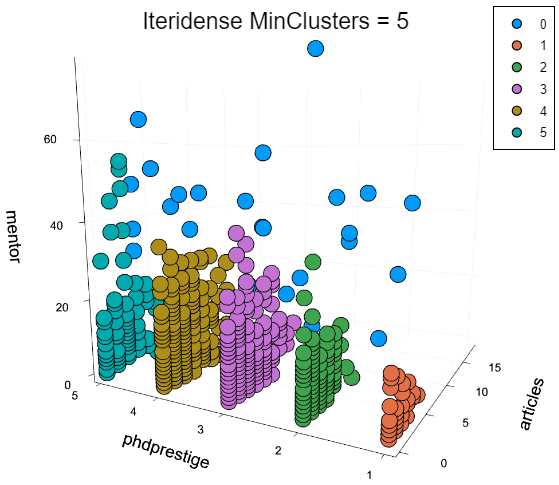
\includegraphics[width=0.45\columnwidth]{clipart/PhdPubs-Iteridense-MinClusters5-sub}
\par\end{centering}
}\hfill{}\subfloat[Evaluation of all 6~dimension]{\begin{centering}
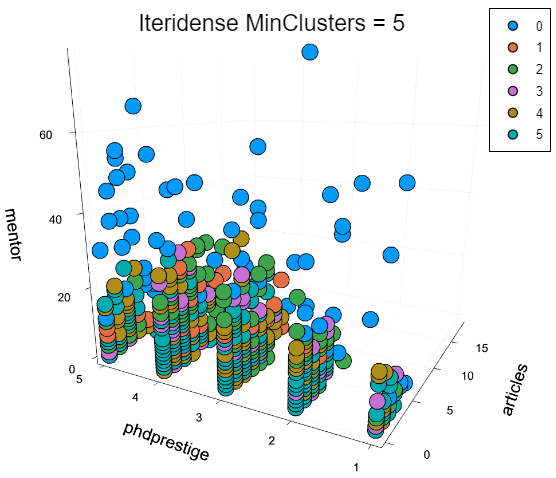
\includegraphics[width=0.45\columnwidth]{clipart/PhdPubs-Iteridense-MinClusters5-complete}
\par\end{centering}
}
\par\end{centering}
\caption{\label{fig:Result-Iteridense-PhD}Result of \noun{Iteridense} on the
\emph{PhDPublications} dataset.}
\end{figure}


\section{Discussion}

As shown in the previous sections, the \noun{Iteridense} algorithm
is applicable for general purposes. It is more computation-efficient
than pure density-based algorithms that evaluate neighboring data
points. But it shares with density-based algorithms the drawback that
clusters overlapping each other cannot be detected. For example it
will perform as poor as DBSCAN on Fisher's Iris data set~\cite{Fisher1936}.

\noun{Iteridense} shows some similarities to the grid-based DENCLUE
algorithm. However, the assignments of the data points to the clusters
is different because\linebreak{}
 DENCLUE assumes a Gaussian distribution function as shape the the
density function. Another big difference to DENCLUE is that there
is not only a single probability-density function created but iteratively
several ones with increasing resolutions. This costs more computation
efforts but one does not have to make assumptions about the density
in the dataset. DENCLUE requires at least 2~input variables. $\xi$
is similar to $\rho$ in \noun{Iteridense}. The parameter $\sigma$
defines the width of the Gaussian that is used to assign the data
points to the clusters. Its value has to be guessed introducing for
some practical applications trial and error. There are approaches
to improve initial the setting of the DENCLUE parameters, see~\cite{Ajmal2024},
but in general this will remain as a practical challenge.

Compared to the grid-based algorithm CLIQUE, \noun{Iteridense} does
not require to specify the size of the cell (CLIQUE's parameter $\xi$)
since the cell width is iteratively approached. There is also no need
to specify the number of data points in a cell to treat the cell as
being part of a cell (CLIQUE's parameter $\tau$). The \noun{Iteridense
}algorithm treats every cell with at least 2~data points as part
of a cluster. This is possible because at the end of every loop (steps~\ref{enu:AlgoStep1}\,--\,\ref{enu:AlgoStep5})
the clusters are evaluated and if their $\rho_{\mathrm{cluster}}$
is too low, the cluster is deleted. This is an advantage to CLIQUE
because especially for high-dimensional data it is hard to estimate
how many data points might end up in a cell.

\noun{Iteridense} is a simple algorithm: The user does not need to
estimate in advance a cell size, how many data points will be in a
cell, the mean distance between data points in a cluster or the like.
One can either specify \textbf{MinClusters} or $\rho$ , sets \textbf{MinClusterSize}
and gets in many cases directly a suitable result. If necessary, \noun{Iteridense}'s
clear path on how to change the input parameters guides the user to
more suitable or different results.

\section{Conclusions}

This paper introduced \noun{Iteridense}, an iterative clustering algorithm
combining grid-based and density-based methods. It is simple to use
because it does not require to estimate settings in advance and because
it provides two possibilities to run the clustering and for both a
clear path on how to change the algorithm's input parameters to achieve
suitable results. \noun{Iteridense} is applicable for datasets with
any dimensionality.

The \noun{Iteridense} algorithm provides shorter computation times
than pure density-based algorithms. Compared to pure grid-based algorithms
it has the advantage that the user does not have to make assumptions
on how the grid should be defined or about the shape of the probability-distribution.

It was demonstrated that \noun{Iteridense} performs clustering as
good to the DBSCAN algorithm and for cases of high-dimension datasets
even better.

\noun{Iteridense} provides different options to affect either the
clustering result and to improve the computation time. We provide
online a reference implementation together with an example worksheet,
\cite{Iteridense}, demonstrating the clustering with \noun{Iteridense}
on the datasets shown in this paper.

\printbibliography[heading=bibintoc]

\end{document}
